\chapter{Meetings with external resources}
\section{Meetings with customer}
\begin{table}[H]
\centering
\begin{tabular}{|l|l|}
\hline
\textbf{Date}&\textbf{Agenda}\\\hline
24.01&\\\hline
31.01&\\\hline
07.02&\\\hline
14.02&\\\hline
21.02&\\\hline
%28.02 kunde følte ikke det var nødvendig med møte
%07.03 kunde bortreist
14.03&\\\hline
%21.03 glemte møteinnkalling
28.03&\\\hline
02.04&\\\hline
%09.04 Kina
%16.04 Påske
%25.04 prøvde å få kontakt med kunde
02.05&\\\hline
\end{tabular}
\caption{Overview on meetings with customer}
\end{table}

\section{Meetings with supervisor}
\begin{table}[H]
\centering
\begin{tabular}{|l|l|p{12.6cm}|}
\hline
\textbf{Week \#} & \textbf{Date}&\textbf{Agenda}\\\hline
5& 31.01&Get familiar with supervisor's tasks and what we are to write in the different project documents requested by the subject administration.\\\hline
7 &14.02&Feedback on report, tips on how we could improve our risk analysis and guidance on how to approach customer if he does not provide us with necessary information.\\\hline
9 &27.02& Feedback and questions on mid-term report.\\\hline
11 &14.03& Feedback on report, especially regarding requirement specification and how we are going to represent the development process in the report.\\\hline
13 &03.04&General feedback on report and status update before the team leaves for China.\\\hline
19&&\\\hline
\end{tabular}
\caption{Overview on meetings with supervisor}
\end{table}

\chapter{Example of project documents}


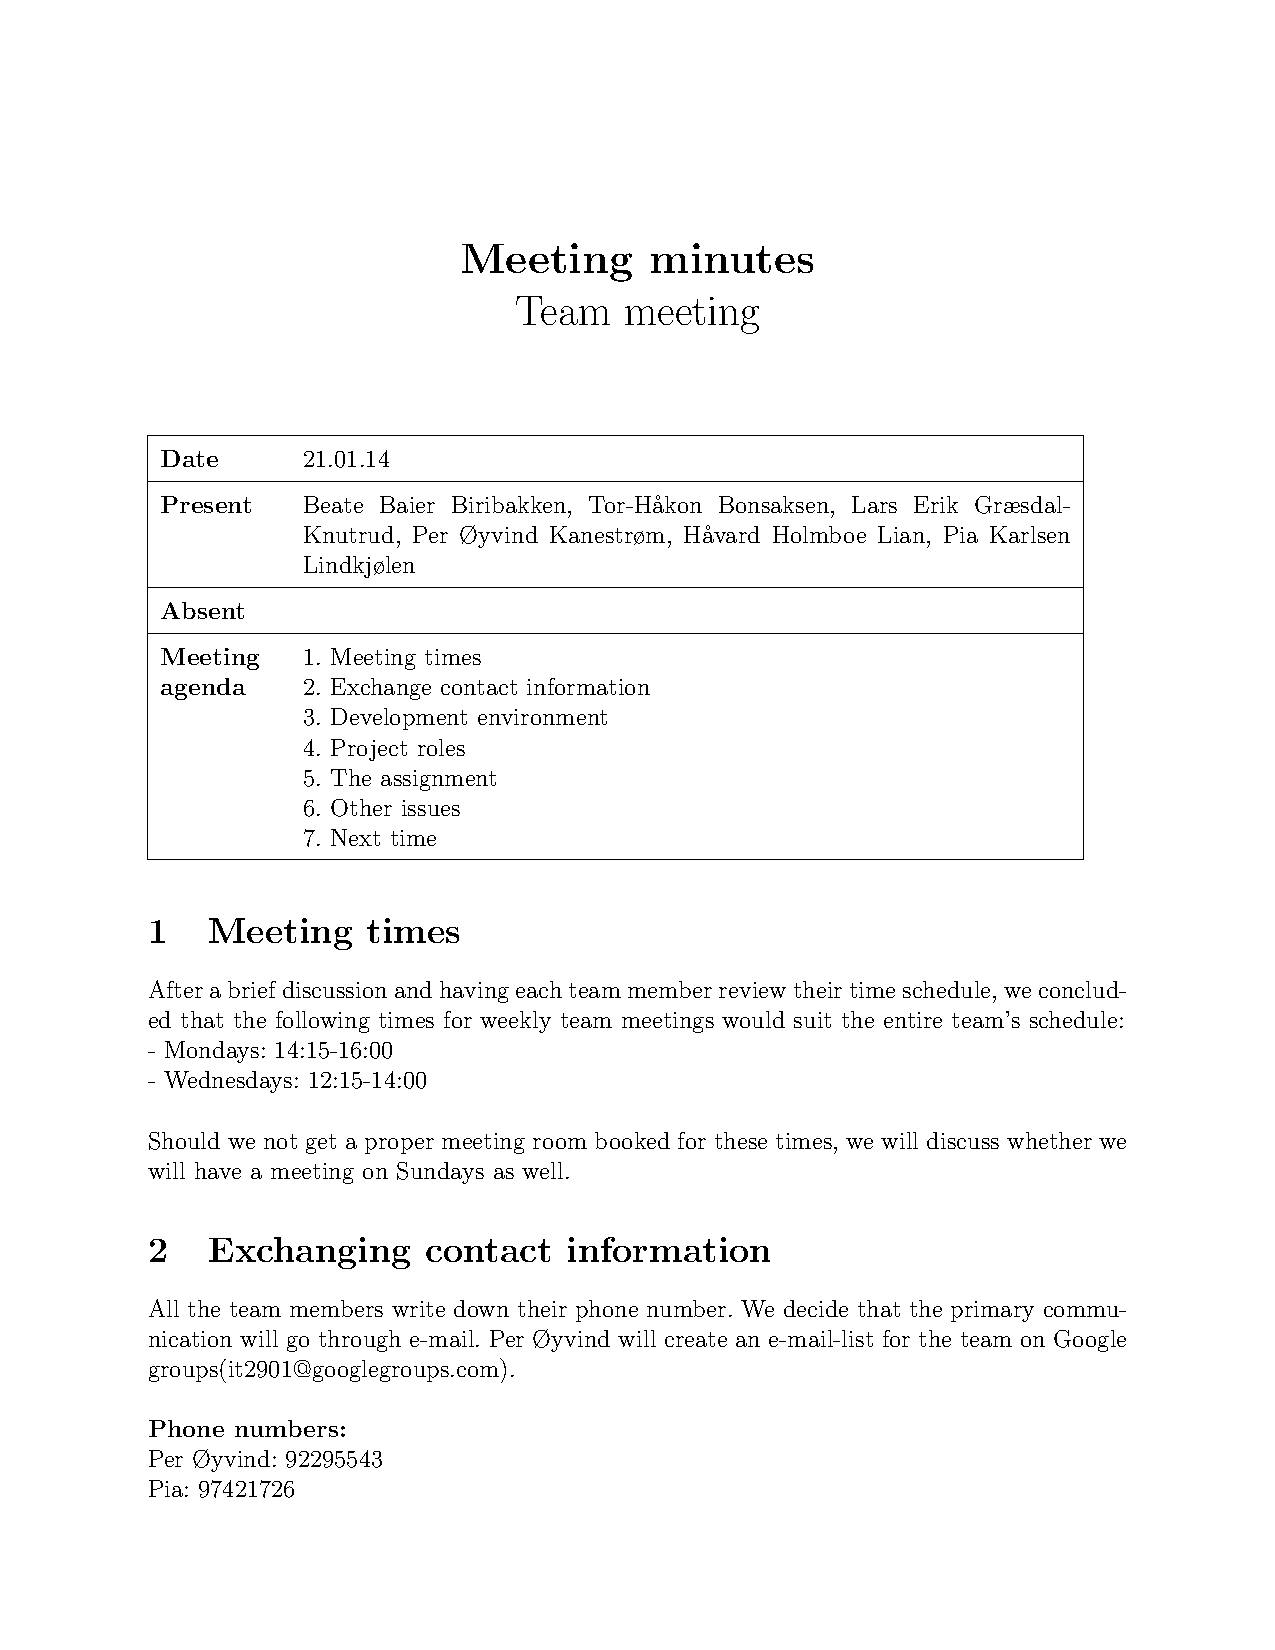
\includepdf[pages=1,pagecommand=\section{Meeting report example}, frame=true, scale=0.76, trim=0mm 10mm 0mm 20mm, clip]{appendix/meetings/firstteammeeting.pdf}
\includepdf[pages=2-3, pagecommand={},fitpaper=true, frame=true, scale=0.76]{appendix/meetings/firstteammeeting.pdf}


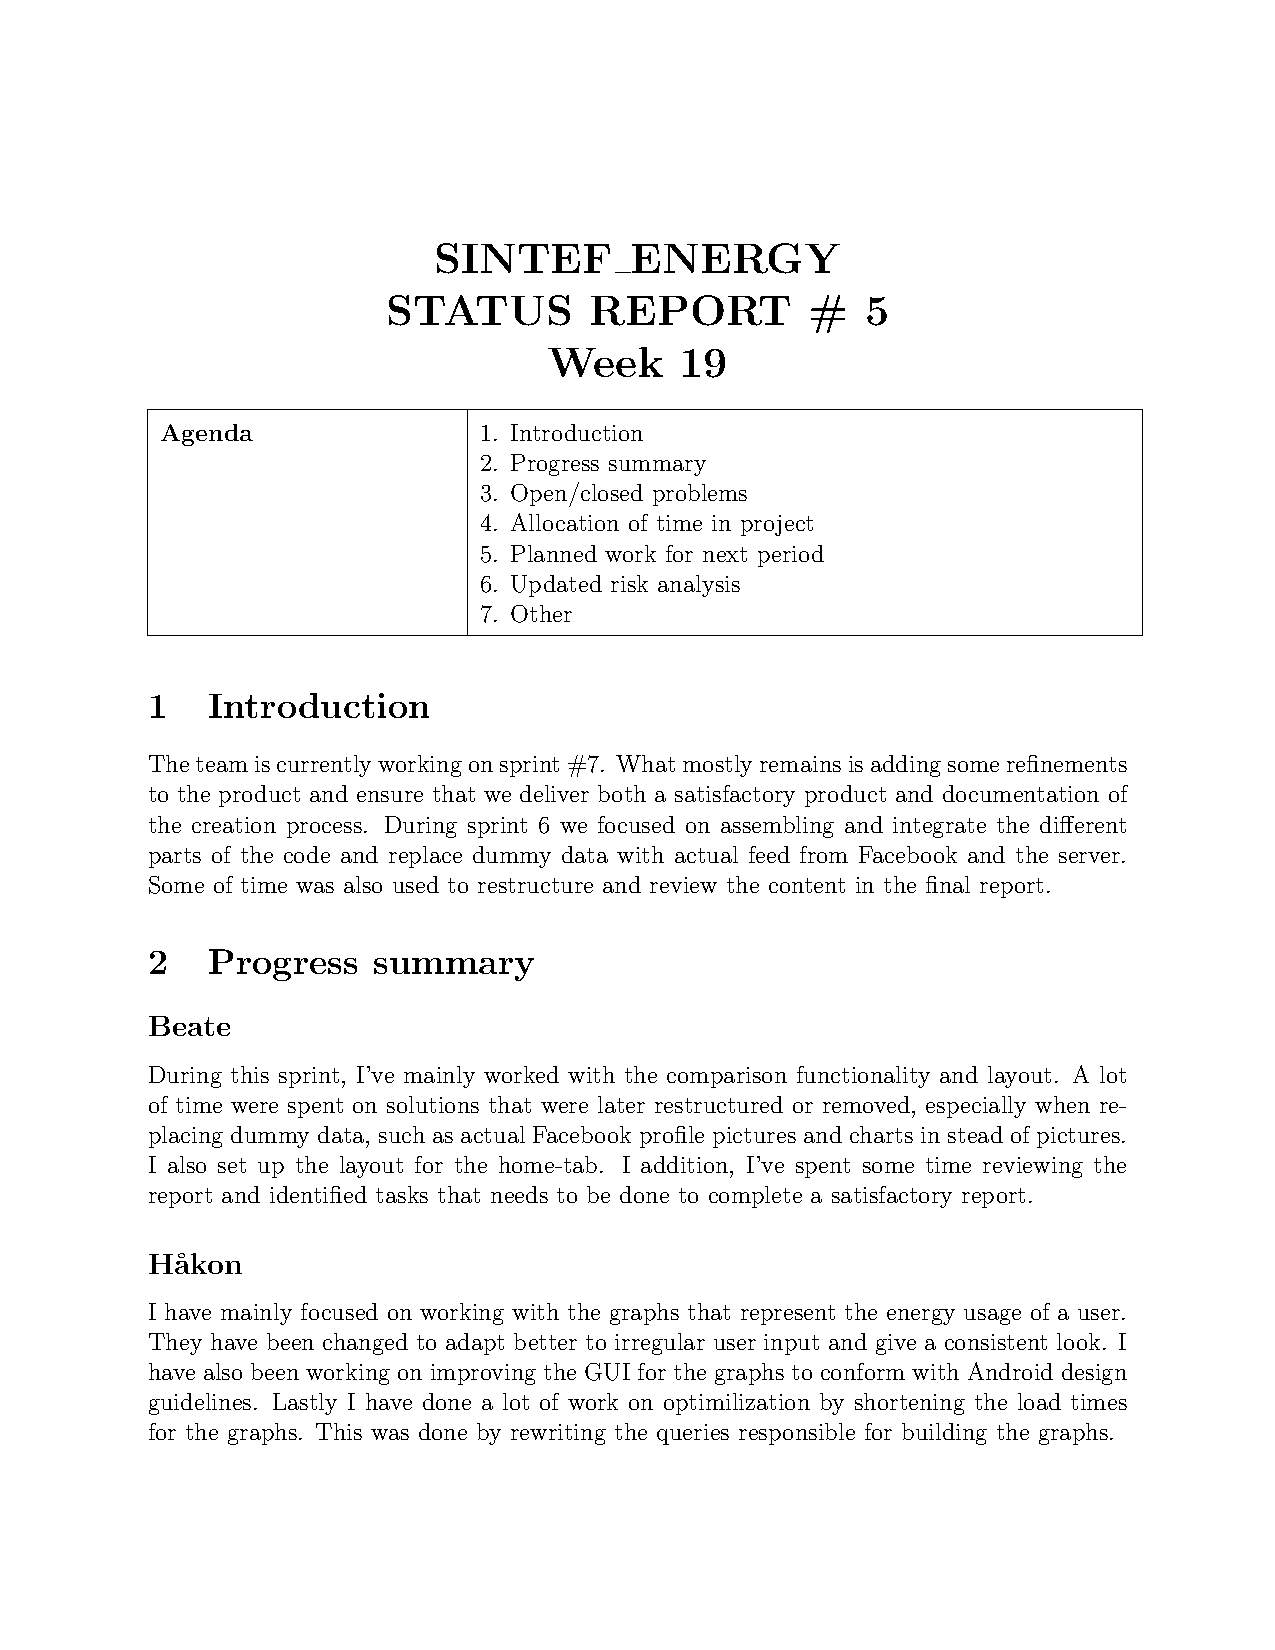
\includepdf[pages=1,pagecommand=\section{Status report example}, frame=true, scale=0.76, trim=0mm 20mm 0mm 20mm, clip]{appendix/meetings/supervisor.pdf}

\includepdf[pages=2,pagecommand={},fitpaper=true, frame=true, scale=0.76]{appendix/meetings/supervisor.pdf}
